% =============================================================================
%  Slides (oral 5 min) — « Combien vaut une voiture d'occasion ? »
%  Introduction to Data Processing — MAM3, Université Côte d'Azur, 2025-2026
%  Équipe : Hafssa, Thibaud, Nathan
%
%  Thème : metropolis (moderne, épuré).
%  Compilation : pdflatex (Overleaf par défaut) ; XeLaTeX/LuaLaTeX pour le vrai Fira.
%  Le script oral est dans les \note{} (afficher avec \setbeameroption{show notes}).
% =============================================================================
\documentclass[aspectratio=169,11pt]{beamer}

\usetheme{metropolis}
\metroset{block=fill, numbering=fraction, progressbar=foot}

\usepackage{iftex}
\ifpdftex
  \usepackage[utf8]{inputenc}
  \usepackage[T1]{fontenc}
\fi
\usepackage[french]{babel}
\usepackage{graphicx}
\usepackage{booktabs}
\usepackage{amsmath,amssymb}
\usepackage{xcolor}

\graphicspath{{figures/}}

% Couleurs : vert = fait MONTER le prix, rouge = fait BAISSER le prix.
\definecolor{priceup}{HTML}{2E7D32}
\definecolor{pricedown}{HTML}{C62828}
\newcommand{\priceUp}[1]{\textcolor{priceup}{#1}}
\newcommand{\priceDn}[1]{\textcolor{pricedown}{#1}}

\title{Combien vaut une voiture d'occasion ?}
\subtitle{Introduction to Data Processing --- MAM3, 2025-2026}
\author{Hafssa \quad\textbullet\quad Thibaud \quad\textbullet\quad Nathan}
\institute{Université Côte d'Azur --- Polytech Nice Sophia}
\date{}

\begin{document}

\maketitle

% ------------------------------------------------------------------ SLIDE 1 --
\begin{frame}{Combien vaut votre voiture d'occasion ?}
  \begin{columns}[T]
    \begin{column}{0.58\textwidth}
      \begin{itemize}
        \item Notre question : \alert{peut-on prédire le prix d'une voiture d'occasion ?}
        \item 1\textsuperscript{er} essai : un dataset « santé mentale » (2\,500 lignes)
          qui ne disait \textbf{rien} ($|r|$ max $\approx 0{,}04$ $\Rightarrow$
          \textbf{synthétique}).
        \item Notre choix : un \textbf{vrai dataset} --- \textbf{72\,000 voitures}
          d'occasion (UK, 7 marques).
        \item Utile : estimer un prix juste, repérer les bonnes affaires, sites
          d'annonces.
      \end{itemize}
    \end{column}
    \begin{column}{0.42\textwidth}
      \centering
      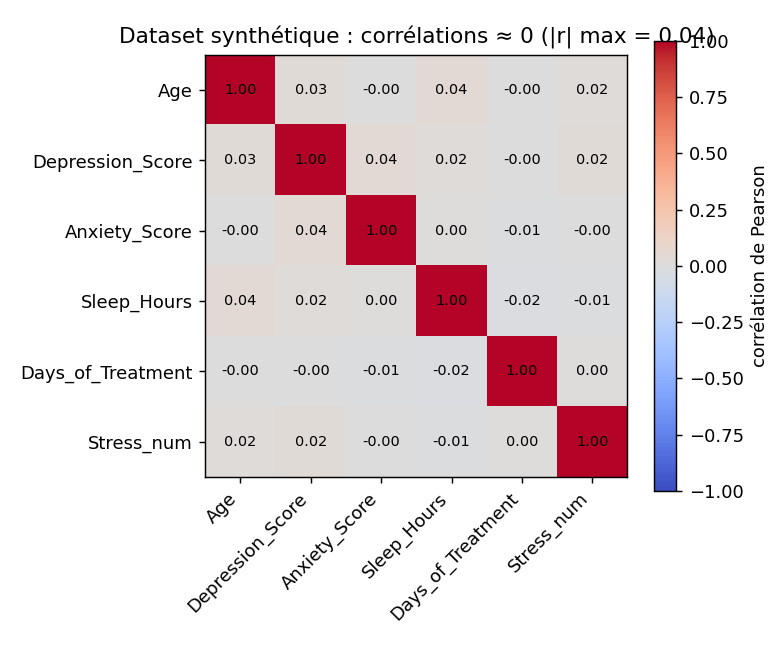
\includegraphics[width=\linewidth]{00_probleme1_synthetique.png}\\
      {\scriptsize Dataset synthétique : corrélations $\approx 0$.}
    \end{column}
  \end{columns}
  \note{On voulait prédire quelque chose d'utile. Premier piège : un dataset « santé
    mentale » parfait en apparence, mais aucune variable n'en expliquait une autre ---
    des données générées artificiellement. On a donc changé pour un vrai dataset :
    72 000 annonces de voitures d'occasion, pour répondre à : combien vaut une voiture ?}
\end{frame}

% ------------------------------------------------------------------ SLIDE 2 --
\begin{frame}{72\,000 voitures, 10 variables, un prix à prédire}
  \begin{columns}[T]
    \begin{column}{0.56\textwidth}
      \begin{itemize}
        \item Source \textbf{réelle} UK Used Cars $\cdot$ \textbf{72\,435 lignes}
          $\cdot$ \textbf{10 variables}.
        \item Cible : \texttt{price}, le prix en \textbf{livres £}.
        \item Numériques : année, kilométrage, taxe, conso, \textbf{cylindrée} ;
          catégorielles : modèle, boîte, carburant, marque.
        \item Nettoyage : années aberrantes (\textbf{2060}, \textbf{1970}) $+$ doublons
          $\to$ \textbf{71\,593 lignes}.
      \end{itemize}
    \end{column}
    \begin{column}{0.44\textwidth}
      \centering
      
\includegraphics[width=\linewidth]{01_heatmap_correlations.png}
    \end{column}
  \end{columns}
  \note{Données réelles : de vraies annonces. On veut prédire le prix. Comme toute vraie
    donnée, elle est imparfaite : une voiture datée de 2060, une de 1970, et des doublons
    --- qu'on a nettoyés. Premier constat sur la heatmap : la cylindrée et l'année
    ressortent.}
\end{frame}

% ------------------------------------------------------------------ SLIDE 3 --
\begin{frame}{2 indices maison à partir de l'année}
  \begin{columns}[T]
    \begin{column}{0.58\textwidth}
      \begin{tabular}{@{}lc@{}}
        \toprule
        \textbf{Feature maison} & \textbf{Corr.\ prix} \\
        \midrule
        \texttt{car\_age} \scriptsize($2026-$année) & \priceDn{$-0{,}52$} \\
        \texttt{mileage\_per\_year} \scriptsize(km $/$ âge) & \priceDn{$-0{,}40$} \\
        \bottomrule
      \end{tabular}
      \medskip
      \begin{itemize}
        \item \texttt{car\_age} : plus une voiture est vieille, moins elle vaut.
        \item \texttt{mileage\_per\_year} : distingue une \textbf{vieille voiture peu
          roulée} d'une \textbf{récente très roulée}.
      \end{itemize}
    \end{column}
    \begin{column}{0.42\textwidth}
      \centering
      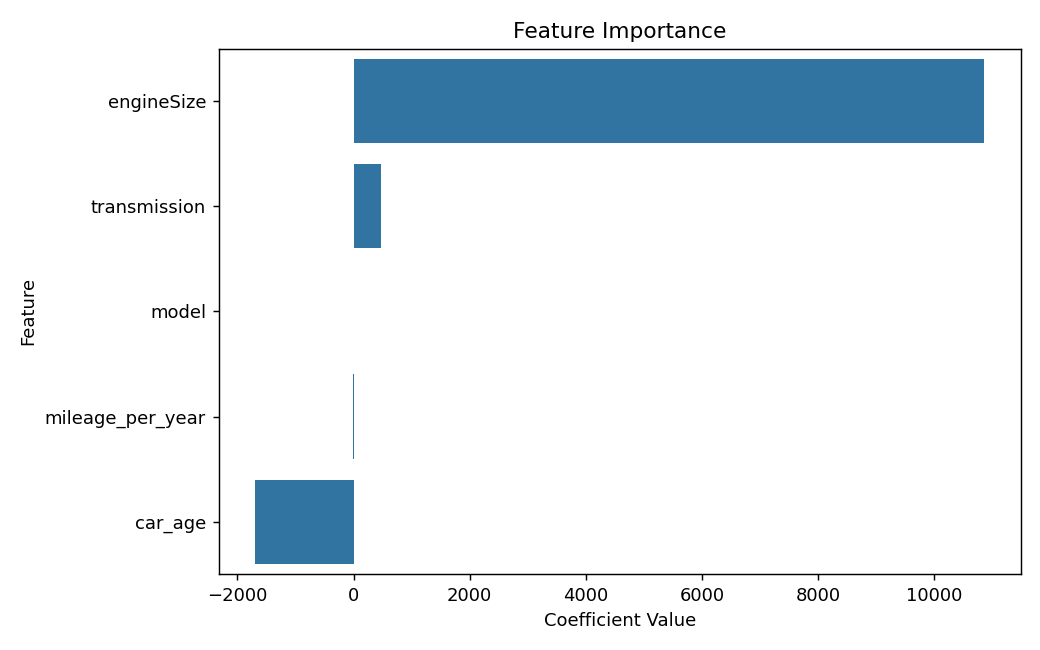
\includegraphics[width=\linewidth]{04_coefficients.png}
    \end{column}
  \end{columns}
  \note{Plutôt que l'année brute, on construit deux indices plus parlants. car\_age,
    l'âge, est notre signal négatif le plus fort (-0.52). Et le kilométrage par an :
    100 000 km, ça n'a pas le même sens sur une voiture de 2 ans ou de 10 ans. Ces deux
    indices simples portent l'effet du temps sur le prix.}
\end{frame}

% ------------------------------------------------------------------ SLIDE 4 --
\begin{frame}{On prédit le prix à 74\,\% --- et on corrige un vrai bug}
  \begin{columns}[T]
    \begin{column}{0.56\textwidth}
      \begin{itemize}
        \item Régression \textbf{linéaire}, 5 variables, split \textbf{80-20}.
        \item \textbf{$R^2$ (test) $=$ 0,735} $\cdot$ $R^2$ (train) $=$ 0,725 (pas de
          surapprentissage) $\cdot$ \textbf{RMSE $\approx$ 4\,800~£}.
        \item \priceUp{\textbf{Monte}} le prix : cylindrée \priceUp{$+10\,862$~£/L},
          boîte $+480$~£.
        \item \priceDn{\textbf{Baisse}} le prix : \priceDn{âge $-1\,695$~£/an},
          km/an $-1{,}3$~£.
        \item \textbf{Bug corrigé} : le code importait $R^2$/RMSE mais ne les
          \textbf{calculait jamais}.
      \end{itemize}
    \end{column}
    \begin{column}{0.44\textwidth}
      \centering
      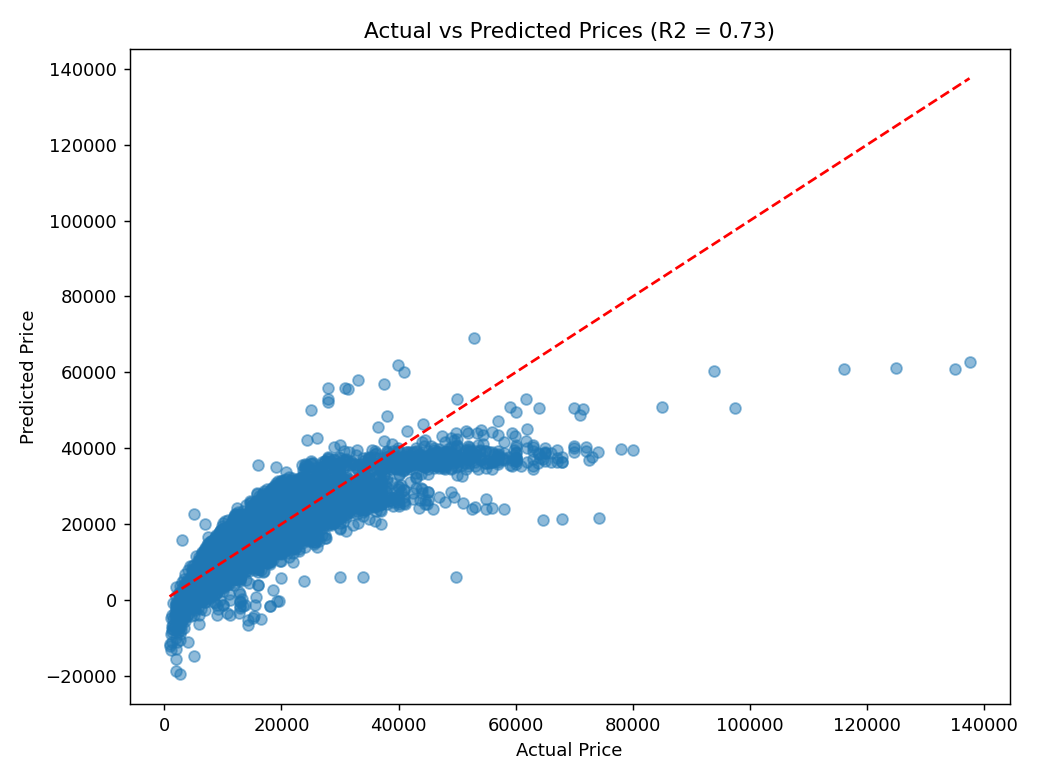
\includegraphics[width=\linewidth]{03_actual_vs_predicted.png}
    \end{column}
  \end{columns}
  \note{Le modèle explique 74 \% du prix --- et train proche de test, donc pas de
    surapprentissage. En moyenne on se trompe de ~4 800 £. Le levier le plus fort, c'est
    la cylindrée ; à l'inverse, chaque année d'âge coûte ~1 700 £. Surtout : le code de
    départ importait le R² et l'erreur mais ne les affichait jamais --- une régression
    qui ne se mesure pas ! On a corrigé ça.}
\end{frame}

% ------------------------------------------------------------------ SLIDE 5 --
\begin{frame}{Des données réelles racontent une histoire --- pas des données fabriquées}
  \begin{itemize}
    \item Un modèle \textbf{simple} explique déjà \textbf{$\sim$74~\%} du prix ; leviers
      clairs (cylindrée $\uparrow$, âge $\downarrow$).
    \item Nos features \texttt{car\_age} / \texttt{mileage\_per\_year} portent l'effet du
      temps.
    \item Leçon : notre 1\textsuperscript{er} dataset (santé mentale) n'expliquait rien
      car \textbf{synthétique} (corrélations $\approx 0$).
    \item Limites : catégories encodées en nombres (faux ordre), prix brut, marque/
      carburant non utilisés.
    \item Pistes : one-hot, modéliser \textbf{$\log(\text{prix})$}, ajouter marque \&
      carburant, Ridge/Lasso.
  \end{itemize}
  \note{En résumé : un modèle simple, mais qui prédit le prix à 74 \% avec des leviers de
    bon sens. Notre plus belle leçon vient de l'échec du début : un dataset fabriqué ne
    raconte rien (corrélations nulles), un dataset réel, si. Savoir faire la différence,
    c'est la première compétence du data scientist. Merci.}
\end{frame}

% ------------------------------------------------------------------- Q&A -----
\begin{frame}{Questions anticipées}
  \footnotesize
  \begin{itemize}
    \item \textbf{Pourquoi linéaire ?} la cible (prix) est \textbf{continue} et on veut
      \textbf{interpréter} les coefficients (en £).
    \item \textbf{$R^2$ de 0,74, c'est bon ?} honnête pour un modèle simple ; et
      \textbf{train $\approx$ test} $\to$ pas de surapprentissage.
    \item \textbf{Pourquoi encoder \texttt{model} en nombre ?} solution \textbf{simple}
      pour un premier modèle ; limite assumée (faux ordre) $\to$ piste $=$ one-hot.
    \item \textbf{Dispersion sur les voitures chères ?} la variance du prix augmente avec
      sa valeur ; piste $=$ modéliser \textbf{$\log(\text{prix})$}.
    \item \textbf{Le vrai bug du code ?} il \textbf{importait} \texttt{r2\_score} /
      \texttt{mean\_squared\_error} mais ne les utilisait jamais $\to$ la régression ne
      s'évaluait pas. Corrigé.
    \item \textbf{Données vraiment réelles ?} vraies annonces UK ; imperfections du réel
      (année 2060, doublons). Le 1\textsuperscript{er} dataset avait des corrélations
      $\approx 0$ $=$ signature du synthétique.
  \end{itemize}
\end{frame}

% ------------------------------------------------------------------ MERCI -----
\begin{frame}[standout]
  Merci !\\[0.5em]
  \small Des données \emph{réelles} racontent une histoire.\\
  \small Des données \emph{fabriquées}, non.
\end{frame}

\end{document}
